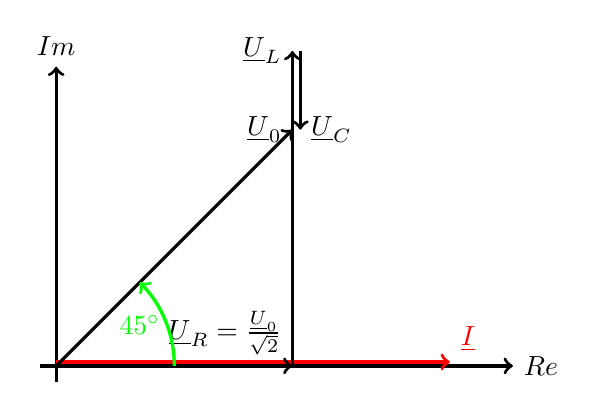
\begin{tikzpicture}
	%Koordinatensystem
	\draw[->, very thick] (-0.2,0) -- +(right:6) node[right] {$Re$};
	\draw[->, very thick] (0,-0.2) -- +(north:4) node[above] {$Im$};
	
	%Pfeile
	\draw[->, color=red, very thick] (0,0.05) -- +(right:5) node[above right]
	{$\underline{I}$};
	\draw[->, very thick] (0,0) -- +(right:3) node[above left] {$\underline{U}_R
	= \frac{\underline{U}_0}{\sqrt{2}}$};
	\draw[->, very thick] (3,0) -- (3,4) node[left]
	{$\underline{U}_L$};
	\draw[->, very thick]	(3.10,4) -- (3.10,3) node[right] {$\underline{U}_C$};
	\draw[->, very thick] (0,0) -- (3,3) node[left] {$\underline{U}_0$};
	
	%Winkel
	\draw[->, very thick, color = green] (1.5,0) arc (0:45:1.5) node[below = 8]
	{$45^{\circ}$};

\end{tikzpicture}


